\sepframe{I. Introduction}

\def\vecwidth{.8}
\def\vecheight{.8}
\tikzset{elem/.style={ultra thick,mybg}}

\begin{frame}
  \frametitle{Structured prediction and NLP}
\begin{itemize}
\item \textbf{Structured prediction}: a machine learning framework for predicting
  structured, constrained, and interdependent outputs
\item \textbf{NLP} deals with \emph{structured} and \emph{ambiguous} textual data:
\begin{itemize}
  \item machine translation
  \item speech recognition
  \item syntactic parsing
  \item semantic parsing
  \item information extraction
  \item ...
\end{itemize}
\end{itemize}
\end{frame}


\begin{comment}
\begin{frame}
  \frametitle{Dependency parsing}

\begin{itemize}
\item Map {\textbf{sentences}} to their {\textbf{syntactic structure.}}
\begin{center}
\only<1->{%
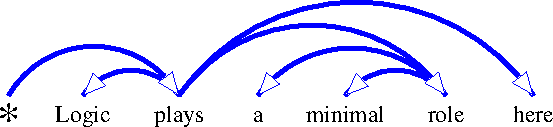
\includegraphics[width=0.6\columnwidth]{img/example_proj_logic01}
}
\end{center}
\begin{itemize}
\item<1-> A lexicalized syntactic formalism
\item<1-> Grammar functions represented as lexical relationships (dependencies)
\end{itemize}
\item[] {\scriptsize{\citep{Eisner1996,McDonald2005b,Nivre2006CoNLL,Koo2007}}}
\end{itemize}
\end{frame}
\end{comment}


\begin{frame}%
\frametitle{Examples of structure in NLP}%
\small%
\makebox[\textwidth][c] {%  center three miniboxes on slide
\onslide<3>%
\begin{minipage}[t][][c]{.31\textwidth}
\centering
{\Large POS tagging}\\
\bigskip
\postag{VERB}{PREP}{NOUN}\\[5.5ex]
\postag{NOUN}{PREP}{NOUN}\\[5.5ex]
\postag{NOUN}{DET}{NOUN}\\
\end{minipage}
\onslide<1->
\begin{minipage}[t][][c]{.40\textwidth}  % 36 min
\centering
{\Large Dependency parsing}\\
\bigskip
$\cdots$\\[1ex]
\simpledep{$\star$ \& dog \& on \& wheels \\}{
\depedge{1}{2}{}
\depedge{2}{3}{}
\depedge{3}{4}{}
}
\\[1ex]
\simpledep{$\star$ \& dog \& on \& wheels \\}{
\depedge{1}{4}{}
\depedge{4}{2}{}
\depedge{4}{3}{}
}
\\[2ex]
\simpledep{$\star$ \& dog \& on \& wheels \\}{
\depedge{1}{2}{}
\depedge{2}{3}{}
\depedge{2}{4}{}
}\\$\cdots$
\end{minipage}
\onslide<3>
\begin{minipage}[t][][c]{.28\textwidth}
\centering
{\Large Word alignments}\\
\bigskip
\matching{2,1,3}
\\[2ex]
\matching{1,2,3}
\\[2ex]
\matching{3,1,2}\\
\end{minipage}}

\onslide<2>\overlaybox{%
\\
\\
{\LARGE Exponentially many parse trees!}\\
\\
{\LARGE Cannot enumerate.}
\\
}

\end{frame}


\begin{frame}[plain]
\frametitle{NLP 5 years ago:}
\framesubtitle{Structured prediction and pipelines}

\begin{center}
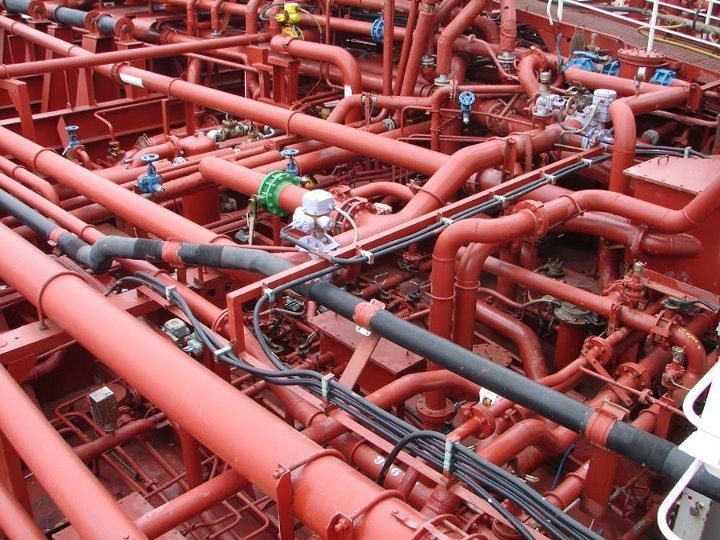
\includegraphics[width=1.\columnwidth]{img/pipeline.jpg}
\end{center}

\end{frame}

\begin{frame}
\frametitle{NLP 5 years ago:}
\framesubtitle{Structured prediction and pipelines}

\begin{itemize}
\item Big pipeline systems, connecting different structured predictors, trained separately
\item {\bf Advantages:} fast and simple to train, can rearrange pieces \emoji{happ}
\item<2-> {\bf Disadvantage:} linguistic annotations required for each component \emoji{sweat}
\item<3-> {\bf Bigger disadvantage:} error propagates through the pipeline \emoji{poop}
\end{itemize}

\end{frame}


\begin{frame}[plain]
\frametitle{NLP today:}
\framesubtitle{End-to-end training}
\begin{center}
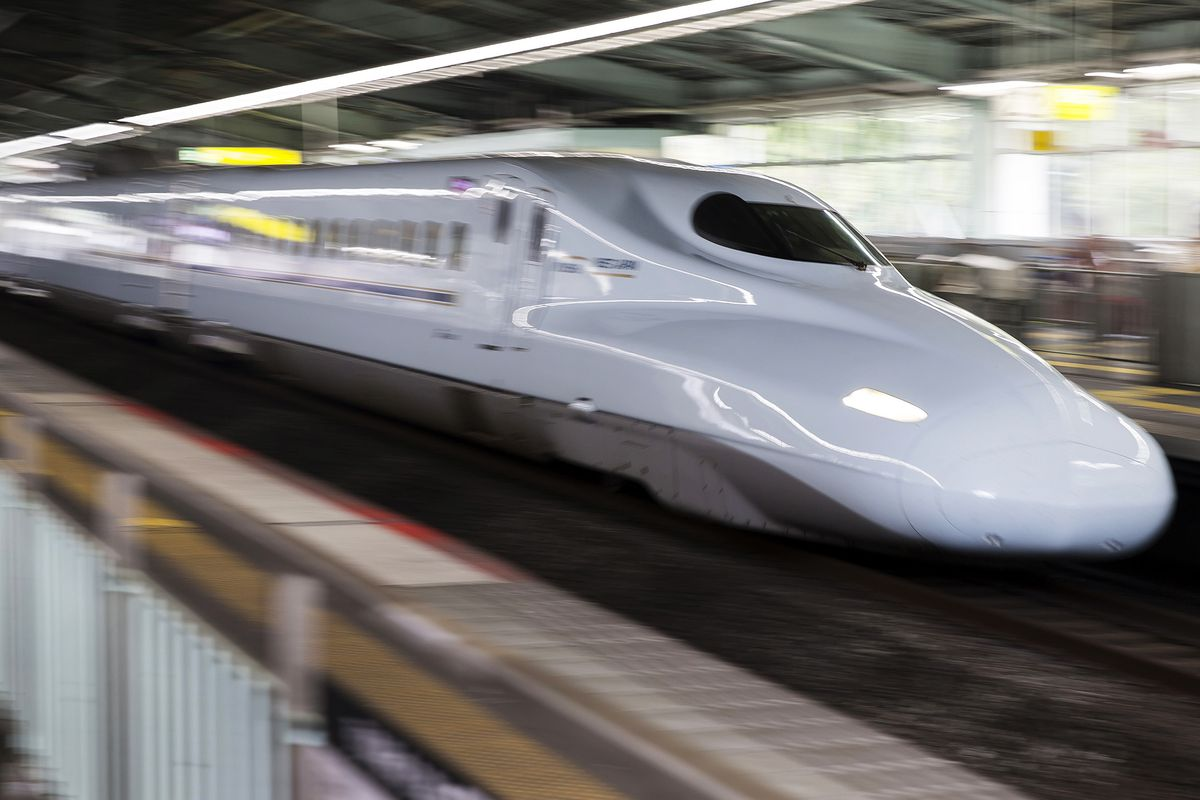
\includegraphics[width=1.\columnwidth]{img/end_to_end_train.jpg}
\end{center}
\end{frame}


\begin{frame}
\frametitle{NLP today:}
\framesubtitle{End-to-end training}

\begin{itemize}
\item Forget pipelines---train everything from scratch!
\item No more error propagation or linguistic annotations! \emoji{party}
\item<2-> Treat everything as \emph{latent}! \emoji{palms}
%\item ... with a little bit of inductive bias to promote the kind of structures we want
\end{itemize}
\end{frame}

%\begin{frame}
%\frametitle{Latent Structure Models}
%
%\begin{itemize}
%\item To be fair, latent structure models were not invented only in the last 5 years.
%\item Example: IBM Models for SMT (latent word alignments).
%\item The ``classical'' approach was based on:
%\begin{itemize}
%\item Generative models trained with the EM algorithm \citep{petrov2008discriminative,ganchev2010posterior}
%\item CRFs with hidden variables \citep{quattoni2007hidden}
%\item Spectral learning and method of moments \citep{hsu2012spectral,anandkumar2012spectral,cohen2012spectral}
%\item Some semi-supervision sometimes \citep{marinho2016semi}
%\end{itemize}
%\item Often, these models make very strict assumptions (e.g. strong factorizations)
%\item Today, neural networks opened up some new possibilities!
%\end{itemize}
%
%\end{frame}


\begin{frame}%
\frametitle{Representation learning}%
\makebox[\textwidth][c] {% two boxes
\begin{minipage}[t][][c]{.45\textwidth}
\begin{itemize}%
\item Uncover hidden representations useful for the \emph{downstream task}.
\item<1-> Neural networks are well-suited for this: \emph{deep computation graphs}.
\item<2-> Neural representations are unstructured, inscrutable. Language data
has underlying structure!
\end{itemize}%
\end{minipage}%
\hfill%
%
\begin{minipage}[t][][c]{.5\textwidth}
\centering
\begin{tikzpicture}[node distance=5pt,inner sep=1pt,scale=.3]
\draw[myfg,thick,fill=mygr!25!mybg] (4.5, 0) rectangle (8.5, 9) {};
\draw[rounded corners,myfg,very thick] (0, 0) rectangle (13, 9) {};
\node[align=center] (In) at (-2, 4.5) {\Huge \faicon{envelope-o}};
\node[align=center] (Out) at (17, 4.5) {\usebox{\sentoutputsmall}};
\node[align=center,above=of In] {\small input};
\node[align=center] at (6.5, 4.5) {}; %{\only<1>{\Huge \faicon{map-o}}};
\path (2.25, 4.5) pic[scale=.25] {cog};
\path (10.75, 4.5) pic[scale=.25] {cog};
%\node[anchor=south west] at (4.5, 0) {$h$};
\only<1->{
\pgfmathsetseed{42}
\foreach \i in {0,1,2,...,8}{
  \pgfmathparse{75*rand}
  \fill[tDY!\pgfmathresult!tPink]  (6, \i) rectangle (7, \i+1) {};
}
\draw[black,thick] (6, 0) rectangle (7, 9) {};
}
\end{tikzpicture}%
\end{minipage}}
\end{frame}
%

\begin{frame}
\frametitle{\only<1->{Latent structure models}}
\makebox[\textwidth][c] {% two boxes
\begin{minipage}[t][][c]{.45\textwidth}
\begin{itemize}%
\item<1-> Seek \emph{structured} hidden representations instead!
\end{itemize}%
\end{minipage}%
\hfill%
%
\begin{minipage}[t][][c]{.5\textwidth}
\centering
\begin{tikzpicture}[node distance=5pt,inner sep=1pt,scale=.3]
\draw[myfg,thick,fill=mygr!25!mybg] (4.5, 0) rectangle (8.5, 9) {};
\draw[rounded corners,myfg,very thick] (0, 0) rectangle (13, 9) {};
\node[align=center] (In) at (-2, 4.5) {\Huge \faicon{envelope-o}};
\node[align=center] (Out) at (17, 4.5) {\usebox{\sentoutputsmall}};
\node[align=center,above=of In] {\small input};
\only<2->{%
\node[align=center,font=\small] at (6.5, 4.5) {%
    $\cdots$\\[-1pt]
    \cartoon[.4]{1/4}\\[1pt]%
    \cartoon[.7]{1/2,1/4}\\[1pt]%
    \cartoon[.4]{2/3,3/4}\\[-3pt]%
    $\cdots$};
}
\path (2.25, 4.5) pic[scale=.25] {cog};
\path (10.75, 4.5) pic[scale=.25] {cog};
%\node[anchor=south west] at (4.5, 0) {$h$};
\only<1>{
\pgfmathsetseed{42}
\foreach \i in {0,1,2,...,8}{
  \pgfmathparse{75*rand}
  \fill[tDY!\pgfmathresult!tPink]  (6, \i) rectangle (7, \i+1) {};
}
\draw[black,thick] (6, 0) rectangle (7, 9) {};
}
\end{tikzpicture}%
\end{minipage}}
\end{frame}

\begin{frame}
\frametitle{Latent structure models aren't so new!}

\begin{itemize}
\item They have a very long history in NLP:
\begin{itemize}
\item IBM Models for SMT (latent word alignments) \citep{brown1993mathematics}
\item HMMs \citep{Rabiner1989}
\item CRFs with hidden variables \citep{quattoni2007hidden}
\item Latent PCFGs \citep{petrov2008discriminative,cohen2012spectral}
\end{itemize}
\item Trained with EM, spectral learning, method of moments, ... \\
%\citep{hsu2012spectral,anandkumar2012spectral,cohen2012spectral,marinho2016semi}
\item Often, very strict assumptions (e.g. strong factorizations)
\item Today, neural networks opened up some new possibilities!
\end{itemize}

\end{frame}


\begin{frame}%
\frametitle{Why do we love latent structure models?}%

\begin{itemize}
\item The inferred latent variables can bring us some {\bf interpretability}
\item They offer a way of injecting prior knowledge as a {\bf structured bias}
\item Hopefully: Higher predictive power with fewer model parameters
\begin{itemize}
\item<2->{\alert{smaller carbon footprint!}}
\end{itemize}
\end{itemize}

\end{frame}


\begin{frame}
\frametitle{What this tutorial is about:}

\begin{itemize}
\item Discrete, combinatorial latent structures
\item Often the structure is inspired by some linguistic intuition
%\item But no supervision beyond this structured induction bias!
\item We'll cover both:
\begin{itemize}
\item RL methods (structure built incrementally, reward coming from downstream task)
\item ... vs end-to-end differentiable approaches (global optimization, marginalization)
\item stochastic computation graphs
\item ... vs deterministic graphs.
\end{itemize}
\item All plugged in \emph{discriminative} neural models.
\end{itemize}
\end{frame}


\begin{frame}
\frametitle{This tutorial is \emph{not} about:}

\begin{itemize}
\item It's not about continuous latent variables
\item It's not about deep generative learning
\item We won't cover GANs, VAEs, etc.
\item There are (very good) recent tutorials on deep variational models for NLP:
\begin{itemize}
\item ``Variational Inference and Deep Generative Models'' (Schulz and Aziz, ACL 2018)
%http://wilkeraziz.github.io/vitutorial.html
\item ``Deep Latent-Variable Models for Natural Language'' (Kim, Wiseman, Rush, EMNLP 2018)
%http://nlp.seas.harvard.edu/latent-nlp-tutorial.html
\end{itemize}
\end{itemize}

\end{frame}


\sepframe[mygr]{Background}

\begin{frame}%
\frametitle{Unstructured vs structured}%

\begin{itemize}
\item To better explain the math, we'll often backtrack to \emph{unstructured} models (where the latent variable is a categorical) before jumping to the \emph{structured} ones
\end{itemize}
\end{frame}


\begin{frame}
\frametitle{The unstructured case: Probability simplex}

\begin{columns}[t]%
\begin{column}{.3\textwidth}%
\begin{tikzpicture}[baseline=(current bounding box.north)]
\setupsimplexbary{}
\coordinate (argmax)    at (barycentric cs:L1=0,L2=0,L3=1);
\coordinate (softmax)   at (barycentric cs:L1=.3,L2=.2,L3=.5);
%\coordinate (sparsemax) at (barycentric cs:L1=.3,L2=0,L3=.7);

\uncover<2->{%
\node[label=west:{\small $[0,0,1]$}] at (argmax) {};
\draw[point,fill=colorArgmax] (argmax) circle[radius=5pt];}
\uncover<3->{%
\node[label=south:{\small $[.3,.2,.5]$}] at (softmax) {};
\draw[point,fill=colorSoftmax] (softmax) circle[radius=5pt];}
\end{tikzpicture}%

\end{column}
\begin{column}{.5\textwidth}%
\begin{itemize}
\item<2-> Each vertex is an \emph{indicator vector}, representing one class:
\begin{equation*}
\z_c = [0, \ldots, 0, \underbrace{1}_{c\text{\textsuperscript{th} position}}, 0, \ldots, 0].
\end{equation*}
\item<3-> Points inside are \emph{probability vectors}, a convex combination of classes:
\begin{equation*}
\p \ge \mathbf{0}, \,\, \sum_c \pp_c = 1.
\end{equation*}
\end{itemize}
\end{column}
\end{columns}

\end{frame}%


\begin{frame}%
\frametitle{What's the analogous of $\triangle$ for a structure?}%

\begin{itemize}
\item A structured object $\bs{z}$ can be represented as a \emph{bit vector}.
\item<2-> Example:
\begin{itemize}
\item<2-> a dependency tree can be represented a $O(L^2)$ vector indexed by arcs
\item<2-> each entry is 1 iff the arc belongs to the tree
\item<2-> {\bf structural constraints:} not all bit vectors represent valid trees!
\end{itemize}
\end{itemize}

\bigskip

\uncover<3->{
\begin{center}
\begin{columns}
\begin{column}{0.3\columnwidth}
\small
$\z_1 = [\textcolor{tPink}{1}, 0, 0, 0, \textcolor{tPink}{1}, 0, 0, 0, \textcolor{tPink}{1}]$\\

\simpledep{$\star$ \& dog \& on \& wheels \\}{
\depedge{1}{2}{}
\depedge{2}{3}{}
\depedge{3}{4}{}
}
\end{column}
\begin{column}{0.3\columnwidth}
\small
$\z_2 = [0, 0, \textcolor{tPink}{1}, 0, 0, \textcolor{tPink}{1}, \textcolor{tPink}{1}, 0, 0]$\\

\simpledep{$\star$ \& dog \& on \& wheels \\}{
\depedge{1}{4}{}
\depedge{4}{2}{}
\depedge{4}{3}{}
}
\end{column}
\begin{column}{0.3\columnwidth}
\small
$\z_3 = [\textcolor{tPink}{1}, 0, 0, 0, \textcolor{tPink}{1}, 0, 0, \textcolor{tPink}{1}, 0]$\\

\simpledep{$\star$ \& dog \& on \& wheels \\}{
\depedge{1}{2}{}
\depedge{2}{3}{}
\depedge{2}{4}{}
}
\end{column}
\end{columns}

\end{center}
}

\end{frame}%

\begin{frame}[label=marginalpoly]%
\frametitle{The structured case: Marginal polytope}%
\cornercite{Wainwright2008}%
\centering

%\begin{itemize}
%\item A structured object $\bs{y}$ (e.g. a dependency tree) can be represented as a \emph{bit vector}.
%\begin{itemize}
%\item e.g. a $O(L^2)$ vector indexed by arcs, where each entry is 1 iff the arc belongs to the tree.
%\end{itemize}
%\end{itemize}

\begin{columns}[t]%
\begin{column}{.7\textwidth}%
\begin{itemize}
    \item<2-> Each vertex corresponds to one such \emph{bit vector} $\z$
    \item<3-> Points inside correspond to \emph{marginal distributions}: convex combinations of structured objects
\begin{equation*}
\mg = \underbrace{{\pp_1} \z_1 + \ldots + {\pp_N} \z_N}_{\text{exponentially many terms}}, \,\, \p \in \Delta.
\end{equation*}

{\small
\begin{equation*}
\begin{array}{ll}
\pp_1 = 0.2, & \z_1 = [\textcolor{tPink}{1}, 0, 0, 0, \textcolor{tPink}{1}, 0, 0, 0, \textcolor{tPink}{1}]\\
\pp_2 = 0.7, & \z_2 = [0, 0, \textcolor{tPink}{1}, 0, 0, \textcolor{tPink}{1}, \textcolor{tPink}{1}, 0, 0]\\
\pp_3 = 0.1, & \z_3 = [\textcolor{tPink}{1}, 0, 0, 0, \textcolor{tPink}{1}, 0, 0, \textcolor{tPink}{1}, 0]\\
\end{array}
\quad \Rightarrow \quad
\mg = [\textcolor{tPink}{.3}, 0, \textcolor{tPink}{.7}, 0, \textcolor{tPink}{.3}, \textcolor{tPink}{.7}, \textcolor{tPink}{.7}, \textcolor{tPink}{.1}, \textcolor{tPink}{.2}].
\end{equation*}
}

%\begin{itemize}
%\item<3-> e.g. each entry $\mu_a$ %= \sum_{\text{tree} \ni a} p(\text{tree})$
%is the marginal probability of arc $a$, given a distribution $\bs{p}$ over trees.
%\end{itemize}
\end{itemize}

\end{column}
\begin{column}[T]{.3\textwidth}%
\centering
\begin{tikzpicture}
\node[
    ultra thick,
    draw=colorPolytope,
    fill=colorPolytope,
    fill opacity=.15,
    minimum size=2.5cm,
    regular polygon, regular polygon sides=6] (mp) {};
\node[label=east:{\small$\mathcal{M}$}] at (mp.corner 5) {};
\foreach \i in {1, ..., 6}%
{
    \draw[colorPolytope,fill] (mp.corner \i) circle[radius=3pt];
}

\onslide<2->{
    \draw[point,fill=colorArgmax] (.6,1.1) circle[radius=5pt];
    \node at (1.5,1) {\cartoon[.5]{1/4,2/5}};
}

\onslide<3->{
    \draw[point,fill=colorSoftmax] (-.2,-.1) circle[radius=5pt];
    \node at (-2, -.5) {\cartoonDense[.5]{}};
}
\end{tikzpicture}
\end{column}
\end{columns}
\end{frame}


\begin{frame}{Unstructured vs Structured}

\begin{columns}[T]%
\begin{column}{.45\textwidth}\centering%
\vbox to .7\textheight{%

\begin{itemize}
\item Unstructured case: simplex $\Delta$
\end{itemize}

\vfill

\begin{tikzpicture}
\setupsimplexbary[2.5]{}
\coordinate (argmax)    at (barycentric cs:L1=0,L2=0,L3=1);
\coordinate (softmax)   at (barycentric cs:L1=.3,L2=.2,L3=.5);
\coordinate (sparsemax) at (barycentric cs:L1=.3,L2=0,L3=.7);

\onslide<2->{
\draw[point,fill=colorArgmax] (argmax) circle[radius=5pt];
}
\onslide<3->{
\draw[point,fill=colorSoftmax] (softmax) circle[radius=5pt];
}
%\onslide<8->{
%\draw[point,fill=colorSparsemax] (sparsemax) circle[radius=5pt];
%}
\end{tikzpicture}}
\end{column}
\begin{column}{.54\textwidth}\centering
\vbox to .7\textheight{%

\begin{itemize}
\item Structured case: marginal polytope $\mathcal{M}$
\end{itemize}

\vfill
\begin{tikzpicture}[node distance=0pt]%
\uncover<1->{
\node[
    ultra thick,
    draw=colorPolytope,
    fill=colorPolytope,
    fill opacity=.15,
    minimum size=2.5cm,
    regular polygon, regular polygon sides=6] (mp) {};
\node[label=east:{\small$\mathcal{M}$}] at (mp.corner 5) {};
\foreach \i in {1, ..., 6}%
{
    \draw[colorPolytope,fill] (mp.corner \i) circle[radius=3pt];
}
}
\coordinate (L1) at (mp.corner 3);
\coordinate (L2) at (mp.corner 5);
\coordinate (L3) at (mp.corner 2);
\coordinate (argmax)    at (L3);
\coordinate (softmax)   at (barycentric cs:L1=.25,L2=.25,L3=.45);
%\coordinate (sparsemax) at (barycentric cs:L1=.4,L3=.6);
\onslide<2->{
    \draw[point,fill=colorArgmax] (argmax) circle[radius=5pt];
    \node[above right=of argmax] {\cartoon[.5]{1/4,2/5}};
}
\onslide<3->{
    \draw[point,fill=colorSoftmax] (softmax) circle[radius=5pt];
    \node[below right=of softmax] {\cartoonDense[.5]{}};
}
%\onslide<9->{
%    \draw[point,fill=colorSparsemax] (sparsemax) circle[radius=5pt];
%    \node[left=of sparsemax] {\cartoonSparse[.5]{}};
%}
\end{tikzpicture}}
\end{column}
\end{columns}

\end{frame}


\begin{frame}
\frametitle{Computing the most likely structure}
\framesubtitle{is a very high-dimensional argmax}
\centering
\begin{tikzpicture}
    \node[anchor=south] at (0, \vecheight*4) {\cartoon[.66]{1/4}};
    \node[anchor=south] at (0, \vecheight*2.5) {\cartoon[.66]{1/2,1/4}};
    \node[anchor=south] at (0, \vecheight*1.5) {$\cdots$};
    \node[anchor=south] at (0, \vecheight*0) {\cartoon[.66]{2/3,2/4}};
\drawscores
\drawargmax[\z]

\node[anchor=south,align=center] at (-6, \vecheight*3+1) (in) {input\\$\bs{x}$};
\node[anchor=south] at (-2, \vecheight*3+1) (in-end) {};
\node[anchor=south,align=center] at (6, \vecheight*3+1)
(out){output\\$\widehat{\bs{y}}$};
\node[anchor=south] at (2, \vecheight*3+1) (out-end) {};
\path (in) edge[->,very thick,bend right=50] (in-end);
\node[anchor=south] at (4, \vecheight*3+.9) (out-mid) {
    \cartoon[.9]{1/2,1/4}
};
\path (out-end) edge[->,very thick,bend right=50] (out-mid.south west);
\path (out-mid.south east) edge[->,very thick,bend right=50] (out);
\end{tikzpicture}

\onslide<2->\overlaybox{%
    There are exponentially\\many structures\\
    {\small ($\s$ cannot fit in memory;}\\
    {\small we cannot ``loop'' over $\s$ nor $\z$)}
}
\end{frame}

\begin{frame}[t,label=structuretypes]%
\frametitle{Dealing with the combinatorial explosion}
\begin{columns}[t]%
\begin{column}{.5\textwidth}%
\centering%
\cartoon[.7]{1/2} $\rightarrow$
\cartoon[.7]{1/2,1/5} $\rightarrow$
\cartoon[.7]{1/2,1/5,1/3} $\rightarrow \cdots$
\\[\baselineskip]
\textbf{1. Incremental structures} \\
\begin{itemize}
\item Build structure \textbf{greedily}, as sequence of discrete choices
(e.g., shift-reduce).
\item Scores (partial structure, action) tuples.
\item {\bf Advantages:} flexible, rich histories.
\item {\bf Disadvantages:} greedy, local decisions are suboptimal,
error propagation.
\end{itemize}
\end{column}
\begin{column}{.5\textwidth}%
\centering%
$\max\big\{\cdots$,
\cartoon[.7]{1/2,1/5,1/3,1/4},
\cartoon[.7]{1/2,1/5,1/3,3/4},
\cartoon[.7]{1/2,1/5,1/3,5/4},
$\cdots\big\}$
\\[\baselineskip]

\textbf{2. Factorization into parts} \\
\begin{itemize}
%\item[] $$ \mg = \bs{A} \p $$
\item Optimizes \textbf{globally} (e.g.\ Viterbi, Chu-Liu-Edmonds,
Kuhn-Munkres).
\item Scores smaller parts.\\
\item {\bf Advantages:} optimal, elegant, can handle hard \& global constraints.
\item {\bf Disadvantages:} strong assumptions.
\end{itemize}
\end{column}
\end{columns}
\end{frame}


\begin{frame}%
\frametitle{The challenge of discrete choices.}%
\centering%
\begin{tikzpicture}
\drawcs
\onslide<2->{\drawscores}
\onslide<3->{\drawargmax[\z]}
%
\onslide<4->{
    \node[anchor=south,align=center] at (-6, \vecheight*3+1) (in) {input\\$\bs{x}$};
\node[anchor=south] at (-2, \vecheight*3+1) (in-end) {};
\node[anchor=south,align=center] at (6, \vecheight*3+1) (out){output\\$\widehat{\bs{y}}$};
\node[anchor=south] at (2, \vecheight*3+1) (out-end) {};
%
\path (in) edge[->,very thick,bend right=50] node[anchor=north] {$\s =
    \bs{f}_{\parp}(\bs{x})$} (in-end);
\path (out-end) edge[->,very thick,bend right=50] node[anchor=north] {$\widehat{\bs{y}} =
    \bs{g}_{\clfp}(\z, \bs{x})$} (out);
}
%
\node at (0, -1) {{%
\onslide<5->{$\frac{\partial L(\widehat{\bs{y}},\bs{y})}{\partial \bs{w}} = ?$}
\onslide<6->{\quad or, essentially, \quad $\frac{\partial \z}{\partial \s}=?$}
}};\end{tikzpicture}
\end{frame}


\begin{frame}%
\frametitle{Discrete mappings are ``flat''}%
\centering%
\begin{tikzpicture}%
%
\node[anchor=south] at (-1-.5*\vecwidth, \vecheight*5+.1) {$\s$};

\drawcs
\drawscores
\drawargmax[\z]

\foreach[count=\i] \x in {64,69,74,79,84,89,94,99}{
    \onslide<\i>{
        \draw[elem,fill=vecfg!\x!vecbg] (-1-\vecwidth, \vecheight*4) rectangle (-1, \vecheight*5);}
}

\node[anchor=south] at (1+.5*\vecwidth, \vecheight*5+.1) {$\z$};
\foreach[count=\i] \x in {64,69,74,79,84,89,94,99}{
\onslide<\i>{
\draw[elem,fill=vecfg!%
\ifnum\x<85
    0
\else
    70
\fi!vecbg]  (1, \vecheight*4) rectangle (1+\vecwidth, \vecheight*5);
%
\draw[elem,fill=vecfg!%
\ifnum\x<85
    70
\else
    0
\fi!vecbg] (1, \vecheight*3) rectangle (1+\vecwidth, \vecheight*4);
}}

\node[anchor=south,align=center] at (-6, \vecheight*3+1) (in) {\phantom{input}};
\node[anchor=south,align=center] at (6, \vecheight*3+1) (out) {\phantom{output}};
%
\node at (0, -1) {$\frac{\partial \z}{\partial \s}=?$};
\end{tikzpicture}\end{frame}

\begin{frame}%
\frametitle{Argmax}
\centering%
\begin{tikzpicture}%
%
\drawcs\drawscores\drawargmax[\z]
%
\node at (0, -1) {$\frac{\partial \z}{\partial \s}=\bs{0}$};
\node[anchor=south,align=center] at (-6, \vecheight*2+1) (in) {\phantom{input}};
\node[anchor=south,align=center] at (6, \vecheight*2+1) (out) {\phantom{output}};
\end{tikzpicture}%
\\[-\baselineskip]

\begin{tikzpicture}[overlay]
    \draw[axisline,->] (3, 3) -- (3, 6) node[left] {$\zz_1$};
    \draw[axisline,->] (3, 3) -- (7, 3) node[right]{$\ss_1$};

    \node[axislabel,left] at (3, 3) {$0$};
    \node[axislabel,left] at (3, 5) {$1$};

    \draw[axisline] ($(3,3) + (-\ticksize, 0)$) -- ($(3,3) + (+\ticksize, 0)$);
    \draw[axisline] ($(3,4) + (-\ticksize, 0)$) -- ($(3,4) + (+\ticksize, 0)$);
    \draw[axisline] ($(3,5) + (-\ticksize, 0)$) -- ($(3,5) + (+\ticksize, 0)$);

    \draw[axisline] ($(3,3) + (0, -\ticksize)$) -- ($(3,3) + (0, +\ticksize)$);
    \draw[axisline] ($(4,3) + (0, -\ticksize)$) -- ($(4,3) + (0, +\ticksize)$);
    \draw[axisline] ($(5,3) + (0, -\ticksize)$) -- ($(5,3) + (0, +\ticksize)$);
    \draw[axisline] ($(6,3) + (0, -\ticksize)$) -- ($(6,3) + (0, +\ticksize)$);

    \node[axislabel,below] at (4, 3) {$\ss_2 - 1$};
    \node[axislabel,below] at (5, 3) {$\ss_2$};
    \node[axislabel,below] at (6, 3) {$\ss_2 + 1$};

    \draw[ultra thick,colorArgmax] (3, 3) -- (5,3) ;
    \draw[ultra thick,colorArgmax] (5, 5) -- (7,5) ;
\end{tikzpicture}
\end{frame}


% \begin{frame}%
% \frametitle{Continuous Relaxation via Softmax}
% \centering%
% \begin{tikzpicture}%
% %
% \drawcs\drawscores\drawsoftmax
% \node at (0, -1) {$\frac{\partial \p}{\partial \s}=\operatorname{diag}(\p) - \p\p^\top$};
% \node[anchor=south,align=center] at (-6, \vecheight*2+1) (in) {\phantom{input}};
% \node[anchor=south,align=center] at (6, \vecheight*2+1) (out) {\phantom{output}};
% \end{tikzpicture}
% \\[-\baselineskip]
%
% \begin{tikzpicture}[overlay]
%     \draw[axisline,->] (3, 3) -- (3, 6) node[left] {$p_1$};
%     \draw[axisline,->] (3, 3) -- (7, 3) node[right]{$\theta_1$};
%
%     \node[axislabel,left] at (3, 3) {$0$};
%     \node[axislabel,left] at (3, 5) {$1$};
%
%     \draw[axisline] ($(3,3) + (-\ticksize, 0)$) -- ($(3,3) + (+\ticksize, 0)$);
%     \draw[axisline] ($(3,4) + (-\ticksize, 0)$) -- ($(3,4) + (+\ticksize, 0)$);
%     \draw[axisline] ($(3,5) + (-\ticksize, 0)$) -- ($(3,5) + (+\ticksize, 0)$);
%
%     \draw[axisline] ($(3,3) + (0, -\ticksize)$) -- ($(3,3) + (0, +\ticksize)$);
%     \draw[axisline] ($(4,3) + (0, -\ticksize)$) -- ($(4,3) + (0, +\ticksize)$);
%     \draw[axisline] ($(5,3) + (0, -\ticksize)$) -- ($(5,3) + (0, +\ticksize)$);
%     \draw[axisline] ($(6,3) + (0, -\ticksize)$) -- ($(6,3) + (0, +\ticksize)$);
%
%     \node[axislabel,below] at (4, 3) {$\theta_2 - 1$};
%     \node[axislabel,below] at (5, 3) {$\theta_2$};
%     \node[axislabel,below] at (6, 3) {$\theta_2 + 1$};
%
%     \draw[ultra thick,colorArgmax] (3, 3) -- (5,3) ;
%     \draw[ultra thick,colorArgmax] (5, 5) -- (7,5) ;
%
%     \draw (3, 3.1) edge[colorSoftmax,ultra thick,out=360,in=180,looseness=1.5] (7, 4.9);
%
%     \node[anchor=south,align=center] at (-5, 4) (in) {$p_j = \exp(\theta_j) / Z$};
%     %\node[anchor=south,align=center] at (-5, 4) (in) {$p_j \coloneqq \exp(\theta_j) / Z$};
%
% \end{tikzpicture}%
% \end{frame}


\begin{frame}%
\colorlet{patcol}{black!60!white}
\tikzset{
    nosep/.style = {inner sep=0, outer sep=0},
    vec/.style = {draw,rectangle,minimum width=5pt,minimum height=30pt},
    wva/.style = {fill=mygr},
    wvb/.style = {fill=mygr},
    grad/.style = {color=tGreen,very thick},
    nograd/.style = {color=tPink,very thick},
    fwd/.style = {very thick, color=mygr}
}
\frametitle{Example: Regression with latent categorization}%
\centering%
{
\pgfdeclarelayer{bg}    % declare background layer
\pgfsetlayers{bg,main}  % set the order of the layers (main is the standard layer)
\begin{tikzpicture}

\uncover<1->{\drawscores}
\uncover<2-11>{\drawargmax[\z]}
\uncover<12>{\drawsoftmax}
%
\node[anchor=north,align=center] at (-6, \vecheight*1+3) (in)
{{\small input $\bs{x}$} \\ \faicon{envelope-o}};

%%% Left half
%%%%%%%%%%%%%

% h vector
\node[vec,wva,right=of in,outer sep=5pt,label={\small $\bs{u}$}] (h) {};

% embedding matrix
\node[below=60pt of in,align=center,anchor=south] (embed)
    {\faListAlt\\[-.25\baselineskip]{\small embeddings $\bs{E}$}};
% w_theta
\node[right=of embed.south east,anchor=south west] (wth) {\small $\bs{W}_{\s}$};

% arrows among left half
\node[right=45pt of h] (in-end) {};
\begin{pgfonlayer}{bg}
\path (in) edge[fwd,->] node[nosep] (inhmid) {} (h);
\path (h) edge[fwd,->] node[nosep] (inthetamid) {} (in-end);
\path (embed) edge[fwd,bend left=25] (inhmid);
\path (wth) edge[fwd,bend left=30] (inthetamid);
\end{pgfonlayer}

% Bottom left
\node [nosep,below=10pt of embed.south,anchor=north,minimum height=20pt] {\small $\bs{u} = \frac{1}{|\bs{x}|} \sum_j \bs{E}_{x_j}$};
\node [nosep,below=10pt of wth.south,anchor=north,minimum height=20pt]
(thetadef) {\small $\s =  \bs{W}_{\s} \bs{u}$};

%%% Right half
%%%%%%%%%%%%%%

\uncover<3->{%
\node[anchor=north,minimum height=20pt,text depth=20pt,align=center] at (+6, \vecheight*1+3) (out)
{\small output $\hat{y}$};
\node[vec,wvb,left=of out,outer sep=5pt,label={\small $\bs{v}$}] (g) {};
\node[left=40pt of g] (out-end) {};

% arrows among right
\path (out-end) edge[fwd,->] node[nosep] (pgmid) {} (g);
\path (g) edge[fwd,->] node[nosep] (gymid) {} (out);

\node[below=60pt of pgmid,anchor=north] (wg) {\small $\bs{W}_{\bs{v}}$};
\node[below=60pt of gymid,anchor=north] (wy) {\small $\bs{W}_y$};

\node [nosep,right=60pt of thetadef,minimum height=20pt] (glbl)
    {\small $\bs{v} = \operatorname{tanh}\left(%
\bs{W}_{\bs{v}}[\bs{u}, \alt<12>{\p}{\z}]
%\alt<12>{\p}{\z}^\top \bs{W}_{\bs{g}})
%{\bs{h}}
\right)$};
\node [nosep,right=90pt of glbl.west,minimum height=20pt] (ylbl) {\small $\hat{y} = \bs{W}_y \bs{v}$};
\node [nosep,right=40pt of ylbl.west,minimum height=20pt] (loss) {\small $L =
%
\only<10>{\textcolor{tGreen}{\EE_{\z}}}
%
(\hat{y} - y)^2$};
}
\uncover<8>{
    \node[tGreen,above=-8pt of loss.north east] (semisuploss)
        {\small $-\log \frac{\exp({\ss}_c)}{Z}$};
%        \path (semisuploss) edge[grad,->,bend left=5] (wth);
%        \path (semisuploss) edge[grad,->,bend left=5] (embed);
}

\begin{pgfonlayer}{bg}
\uncover<2->{\node[anchor=south] at (.5, \vecheight*3) {\small $(c)$};}

% this line go away when we reparametrize
\uncover<3->{%
\path (h) edge[fwd, bend left=20] (pgmid);
\path (wg) edge[fwd,bend left=30] (pgmid);
\path (wy) edge[fwd,bend left=30] (gymid);
}

\uncover<4->{%
\node[below=5pt of out.west,nosep] (gradorigin) {};
\node[below=5pt of pgmid,nosep] (gradpgmid) {};
\node[below=5pt of inthetamid,nosep] (gradinthetamid) {};
\node[above=0pt of pgmid] (gradpgmidtop) {};
\node[above=5pt of h.east] (gradh) {};
\node[below=10pt of inhmid] (gradinhmid) {};
\path (gradorigin) edge[grad,->,bend right=20] (wy);
\path (gradorigin) edge[grad] (gradpgmid);
\path (gradpgmid) edge[grad,->,bend right=20] (wg);
\path (h) edge[grad,->,bend right=15] (embed);
}
% this line goes away when we reparametrize
\uncover<4-8>{%
\path (gradpgmidtop) edge[grad,->, bend right=20] (gradh);
}
\uncover<5-9>{
\path (gradpgmid) edge[nograd] (gradinthetamid);
\path (gradinthetamid) edge[nograd,->,bend right=20] (wth);
}
\uncover<8>{
\path (.5, \vecheight*3) edge[grad,dashed,->,bend right=20] (wth);
}
%\uncover<9-10>{
%\node[right=10pt of in-end] (threp) {};
%\path (threp) edge[fwd,dashed,bend left=20] (g.west);
%\path ([yshift=5pt]g.west) edge[grad,dashed,->,bend right=20] ([yshift=5pt]threp);
%\path (in-end) edge[grad,dashed,->,bend right=20] (wth);
%}
\uncover<10->{
\path (gradpgmid) edge[grad] (gradinthetamid);
\path (gradinthetamid) edge[grad,->,bend right=20] (wth);
}
\end{pgfonlayer}
\uncover<5>{
    \node[draw,minimum width=20pt,tPink,rectangle] (wthborder) at (wth) {};
}
\end{tikzpicture}
}%
\\[.5\baselineskip]
\begin{overlayarea}{\linewidth}{3\baselineskip}
\centering%
\only<2-3>{predict topic $c$ ($\bs{z} = \bs{e}_c$)}
\only<5>{%
\small
$\pfrac{L}{\bs{W}_{\s}}=
\pfrac{L}{\hat{y}}~
\pfrac{\hat{y}}{\bs{v}}~
\pfrac{\bs{v}}{\bs{z}}
\overbrace{\textstyle\textcolor{tPink}{\pfrac{\z}{\s}}}^{\equiv 0}
\pfrac{\s}{\bs{W}_{\s}}
$}
\only<7>{Option 1. Pretrain latent classifier $\bs{W}_{\s}$}
\only<8>{Option 2. Multi-task learning}
%\only<9>{Option 3. Parameter sharing}
%\only<10>{Option 2+3. Multi-task learning}
\only<10>{Option 3. Stochasticity! $\pfrac{\EE_{\z} (\hat{y}(\z) -
y)^2}{\bs{W}_{\ss}} \neq \bs{0}$}
\only<11>{Option 4. Gradient surrogates (\emph{e.g.} straight-through,
${\pfrac{\z}{\s}}\leftarrow \bs{I}$)}
\only<12>{Option 5. Continuous relaxation (\emph{e.g.} softmax)}
\end{overlayarea}
\uncover<6>{\overlaybox{Workarounds: circumventing the issue, \\ bypassing
discrete variables}}
\uncover<9>{\overlaybox{Tackling discreteness end-to-end}}
\end{frame}
%
%











%\begin{comment}
%\frametitle{Example: Regression with latent categorization}%
%\centering%
%{
%\pgfdeclarelayer{bg}    % declare background layer
%\pgfsetlayers{bg,main}  % set the order of the layers (main is the standard layer)
%\begin{tikzpicture}
%
%\uncover<1->{\drawscores}
%\uncover<2-11,13>{\drawargmax}
%\uncover<12>{\drawsoftmax}
%%
%\node[anchor=north,align=center] at (-6, \vecheight*1+3) (in)
%{{\small input $\bs{x}$} \\ \faicon{envelope-o}};
%
%%%% Left half
%%%%%%%%%%%%%%
%
%% h vector
%\node[vec,wva,right=of in,outer sep=5pt,label={\small $\bs{h}$}] (h) {};
%
%% embedding matrix
%\node[below=60pt of in,align=center,anchor=south] (embed)
%    {\faListAlt\\[-.25\baselineskip]{\small embeddings $\bs{E}$}};
%% w_theta
%\node[right=of embed.south east,anchor=south west] (wth) {\small $\bs{W}_{\bs{\theta}}$};
%
%% arrows among left half
%\node[right=45pt of h] (in-end) {};
%\begin{pgfonlayer}{bg}
%\path (in) edge[fwd,->] node[nosep] (inhmid) {} (h);
%\path (h) edge[fwd,->] node[nosep] (inthetamid) {} (in-end);
%\path (embed) edge[fwd,bend left=25] (inhmid);
%\path (wth) edge[fwd,bend left=30] (inthetamid);
%\end{pgfonlayer}
%
%% Bottom left
%\node [nosep,below=10pt of embed.south,anchor=north,minimum height=20pt] {\small $\bs{h} = \frac{1}{|\bs{x}|} \sum_j \bs{E}_{x_j}$};
%\node [nosep,below=10pt of wth.south,anchor=north,minimum height=20pt] (thetadef) {\small $\bs{\theta} =  \bs{W}_{\bs{\theta}} \bs{h}$};
%
%%%% Right half
%%%%%%%%%%%%%%%
%
%\uncover<3->{%
%\node[anchor=north,minimum height=20pt,text depth=20pt,align=center] at (+6, \vecheight*1+3) (out)
%{\small output $\hat{y}$};
%\node[vec,wvb,left=of out,outer sep=5pt,label={\small $\bs{g}$}] (g) {};
%\node[left=40pt of g] (out-end) {};
%
%% arrows among right
%\path (out-end) edge[fwd,->] node[nosep] (pgmid) {} (g);
%\path (g) edge[fwd,->] node[nosep] (gymid) {} (out);
%
%\node[below=60pt of pgmid,anchor=north] (wg) {\small $\bs{W}_{\bs{g}}$};
%\node[below=60pt of gymid,anchor=north] (wy) {\small $\bs{W}_y$};
%
%\node [nosep,right=60pt of thetadef,minimum height=20pt] (glbl)
%    {\small $\bs{g} = \operatorname{relu}\left((\bs{p}^\top \bs{W}_{\bs{g}})
%\alt<9-10>{\cancel{\bs{h}}~\textcolor{tGreen}{\bs{\theta}}}{\bs{h}}
%\right)$};
%\node [nosep,right=90pt of glbl.west,minimum height=20pt] (ylbl) {\small $\hat{y} = \bs{W}_y \bs{g}$};
%\node [nosep,right=40pt of ylbl.west,minimum height=20pt] (loss) {\small $\ell =
%%
%\only<13>{\textcolor{tGreen}{\EE_{\bs{p}}}}
%%
%(\hat{y} - y)^2$};
%}
%\uncover<8,10>{
%    \node[tGreen,above=-8pt of loss.north east] (semisuploss)
%        {\small $- \alpha \log \nicefrac{\theta_c}{Z}$};
%%        \path (semisuploss) edge[grad,->,bend left=5] (wth);
%%        \path (semisuploss) edge[grad,->,bend left=5] (embed);
%}
%
%\begin{pgfonlayer}{bg}
%\uncover<2->{\node[anchor=south] at (.5, \vecheight*3) {\small $(c)$};}
%
%% this line go away when we reparametrize
%\uncover<3-8,11->{%
%\path (h) edge[fwd, bend left=20] (pgmid);
%}
%\uncover<3->{%
%\path (wg) edge[fwd,bend left=30] (pgmid);
%\path (wy) edge[fwd,bend left=30] (gymid);
%}
%
%\uncover<4->{%
%\node[below=5pt of out.west,nosep] (gradorigin) {};
%\node[below=5pt of pgmid,nosep] (gradpgmid) {};
%\node[below=5pt of inthetamid,nosep] (gradinthetamid) {};
%\node[above=0pt of pgmid] (gradpgmidtop) {};
%\node[above=5pt of h.east] (gradh) {};
%\node[below=10pt of inhmid] (gradinhmid) {};
%\path (gradorigin) edge[grad,->,bend right=20] (wy);
%\path (gradorigin) edge[grad] (gradpgmid);
%\path (gradpgmid) edge[grad,->,bend right=20] (wg);
%\path (h) edge[grad,->,bend right=15] (embed);
%}
%% this line goes away when we reparametrize
%\uncover<4-8>{%
%\path (gradpgmidtop) edge[grad,->, bend right=20] (gradh);
%}
%\uncover<5-11>{
%\path (gradpgmid) edge[nograd] (gradinthetamid);
%\path (gradinthetamid) edge[nograd,->,bend right=20] (wth);
%}
%\uncover<8,10>{
%\path (.5, \vecheight*3) edge[grad,dashed,->,bend right=20] (wth);
%}
%\uncover<9-10>{
%\node[right=10pt of in-end] (threp) {};
%\path (threp) edge[fwd,dashed,bend left=20] (g.west);
%\path ([yshift=5pt]g.west) edge[grad,dashed,->,bend right=20] ([yshift=5pt]threp);
%\path (in-end) edge[grad,dashed,->,bend right=20] (wth);
%}
%\uncover<12->{
%\path (gradpgmid) edge[grad] (gradinthetamid);
%\path (gradinthetamid) edge[grad,->,bend right=20] (wth);
%}
%\end{pgfonlayer}
%\uncover<5>{
%    \node[draw,minimum width=20pt,tPink,rectangle] (wthborder) at (wth) {};
%}
%\end{tikzpicture}
%}%
%\\[.5\baselineskip]
%\begin{overlayarea}{\linewidth}{3\baselineskip}
%\centering%
%\only<2-3>{predict topic $c$ ($\p = \bs{e}_c$)}
%\only<5>{%
%\small
%$\pfrac{\ell}{\bs{W}_{\bs{\theta}}}=
%\pfrac{\ell}{\hat{y}}~
%\pfrac{\hat{y}}{\bs{g}}~
%\pfrac{\bs{g}}{\bs{p}}
%\overbrace{\textstyle\textcolor{tPink}{\pfrac{\bs{p}}{\bs{\theta}}}}^{\equiv 0}
%%\overbrace{\textstyle \pfrac{\bs{p}}{\bs{\theta}}}^{\equiv 0}~
%\pfrac{\bs{\theta}}{\bs{W}_{\bs{\theta}}}
%$}
%\only<7>{Option 1. Pretrain latent classifier $\bs{W}_{\bs{\theta}}$}
%\only<8>{Option 2. Semi-supervision}
%\only<9>{Option 3. Parameter sharing}
%\only<10>{Option 2+3. Multi-task learning}
%\only<12>{Option 5. Continuous relaxation (\emph{e.g.} softmax)}
%\only<13>{Option 6. Stochasticity! $\pfrac{\EE_{\p} (\hat{y} -
%y)^2}{\bs{W}_{\bs{\theta}}} \neq \bs{0}$}
%\end{overlayarea}
%\uncover<6>{\overlaybox{Workarounds: circumventing the issue, \\ bypassing
%discrete variables}}
%\uncover<11>{\overlaybox{Tackling discreteness end-to-end}}
%\end{frame}
%%
%%
%\end{comment}

\begin{frame}%
\frametitle{Dealing with discrete latent variables}%

\begin{center}
\begin{enumerate}
\item Pre-train external classifier
\item Multi-task learning
\item \alert<2->{Stochastic latent variables} \uncover<2->{\alert{(Part 2)}}
\item \alert<2->{Gradient surrogates} \uncover<2->{\alert{(Part 3)}}
\item \alert<2->{Continuous relaxation} \uncover<2->{\alert{(Part 4)}}
\end{enumerate}
\end{center}

\end{frame}

%\begin{frame}%
%\frametitle{Bypassing Latent Variables: External Classifier}%
%\centering
%\end{frame}
%
%\begin{frame}%
%\frametitle{Bypassing Latent Variables: Transfer Learning}%
%\centering
%\end{frame}
%
%\begin{frame}%
%\frametitle{Bypassing Latent Variables: Multi-Task Learning}%
%\centering
%\end{frame}
%


%\begin{frame}%
%\frametitle{Challenges}%
%\centering
%\end{frame}


%\begin{frame}
%\frametitle{Structured Prediction}
%\only<2->{\framesubtitle{is essentially  a (very high-dimensional) argmax}}
%\centering
%\begin{tikzpicture}
%\only<3>{\drawcs}
%\only<4->{
%    \node[anchor=south] at (0, \vecheight*4) {\cartoon[.66]{1/4}};
%    \node[anchor=south] at (0, \vecheight*2.5) {\cartoon[.66]{1/2,1/4}};
%    \node[anchor=south] at (0, \vecheight*1.5) {$\cdots$};
%    \node[anchor=south] at (0, \vecheight*0) {\cartoon[.66]{2/3,2/4}};
%}
%\only<3->{%
%\drawscores
%\drawargmax
%
%\node[anchor=south,align=center] at (-6, \vecheight*3+1) (in) {input\\$\bs{x}$};
%\node[anchor=south] at (-2, \vecheight*3+1) (in-end) {};
%\node[anchor=south,align=center] at (6, \vecheight*3+1) (out){output\\$\bs{y}$};
%\node[anchor=south] at (2, \vecheight*3+1) (out-end) {};
%\path (in) edge[->,very thick,bend right=50] (in-end);
%\node[anchor=south] at (4, \vecheight*3+.9) (out-mid) {
%    \alt<3>{$c_2$}{\cartoon[.9]{1/2,1/4}}
%};
%\path (out-end) edge[->,very thick,bend right=50] (out-mid.south west);
%\path (out-mid.south east) edge[->,very thick,bend right=50] (out);
%}
%\end{tikzpicture}
%
%\onslide<5->\overlaybox{%
%    There are exponentially\\many structures\\
%    {\small ($\s$ cannot fit in memory;}\\
%    {\small we cannot ``loop'' over $\s$ nor $\p$)}
%}
%\end{frame}
%
%\begin{frame}[t]%
%\frametitle{Dealing with the combinatorial explosion}
%%\framesubtitle{Two main strategies:}
%\begin{columns}[t]%
%\begin{column}{.5\textwidth}%
%\centering%
%\textbf{1. Factorization into parts} \\
%\begin{itemize}
%\item $$ \mg = \bs{A} \p $$
%\item Assigns a score to the smaller parts that make up a structure
%\item Optimizes \textbf{globally}
%\item Advantages: optimal, elegant, can handle hard \& global constraints
%\item Disadvantages: relies on discrete optimization algorithms
%(e.g.\ Viterbi, Hungarian)
%\end{itemize}
%\end{column}
%\begin{column}{.5\textwidth}%
%\centering%
%\textbf{2. Incremental structures} \\
%\begin{itemize}
%\item Build a structure through a sequence of discrete choices
%(e.g., shift-reduce)
%\item Formalized as assigning a score to any (partial structure, action) tuple.
%\item Advantages: often simpler to code, allows expressive scoring
%\item Disadvantages: local decisions suboptimal in retrospect,
%no global constraints,
%advanced versions become expensive (imitation learning)
%\end{itemize}
%\end{column}
%\end{columns}
%\end{frame}




\begin{frame}%
\frametitle{Roadmap of the tutorial}%

\begin{itemize}
\item Part 1: Introduction $\checkmark$
\item Part 2: Reinforcement learning
\item Part 3: Gradient surrogates
\item[]
\item[] \emph{Coffee Break}
\item[]
\item Part 4: End-to-end differentiable models
\item Part 5: Conclusions
\end{itemize}

\end{frame}


